\documentclass[12pt,a4paper,UTF8]{ctexart}
\usepackage{graphicx}
\usepackage{amsmath}
\usepackage{amssymb}
\usepackage{cite}
\usepackage[ntheorem]{empheq}
\usepackage{enumitem}
\usepackage{fullpage}
\usepackage{tocbibind}
\usepackage[bookmarksopen=true,colorlinks,linkcolor=black]{hyperref}
\usepackage{cellspace}
\usepackage{listings}
\usepackage{color}
\usepackage{epstopdf}
\usepackage{subfigure}
\usepackage{algorithm}
\usepackage{algorithmicx}
\usepackage{algpseudocode}
\usepackage{lipsum}
\usepackage[thmmarks,amsmath]{ntheorem}



\theoremstyle{nonumberplain}

\theoremheaderfont{\bfseries}

\theorembodyfont{\normalfont}

\theoremsymbol{$\square$}

\newtheorem{Proof}{\hskip 2em 证明}


\makeatletter
\newenvironment{breakablealgorithm}
  {% \begin{breakablealgorithm}
   \begin{center}
     \refstepcounter{algorithm}% New algorithm
     \hrule height.8pt depth0pt \kern2pt% \@fs@pre for \@fs@ruled
     \renewcommand{\caption}[2][\relax]{% Make a new \caption
       {\raggedright\textbf{\ALG@name~\thealgorithm} ##2\par}%
       \ifx\relax##1\relax % #1 is \relax
         \addcontentsline{loa}{algorithm}{\protect\numberline{\thealgorithm}##2}%
       \else % #1 is not \relax
         \addcontentsline{loa}{algorithm}{\protect\numberline{\thealgorithm}##1}%
       \fi
       \kern2pt\hrule\kern2pt
     }
  }{% \end{breakablealgorithm}
     \kern2pt\hrule\relax% \@fs@post for \@fs@ruled
   \end{center}
  }
\makeatother
\renewcommand{\algorithmicrequire}{\textbf{Input:}}  % Use Input in the format of Algorithm
\renewcommand{\algorithmicensure}{\textbf{Output:}} % Use Output in the format of Algorithm
\usepackage{longtable}

\usepackage{float}
\definecolor{gray}{rgb}{0.5,0.5,0.5}
\definecolor{dkgreen}{rgb}{.068,.578,.068}
\definecolor{dkpurple}{rgb}{.320,.064,.680}

% set Matlab styles
\lstset{
   language=Matlab,
   numbers=left,
   keywords={break,case,catch,continue,else,elseif,end,for,function,
      global,if,otherwise,persistent,return,switch,try,while},
   basicstyle=\ttfamily,
   keywordstyle=\color{blue}\bfseries,
   commentstyle=\color{dkgreen},
   stringstyle=\color{dkpurple},
   backgroundcolor=\color{white},
   breaklines=true,
   tabsize=4,
   showspaces=false,
   showstringspaces=false,
}

\begin{document}
\CJKfamily{zhkai}


\begin{center}
    \textbf{作业二}\\
    \textbf{姓名 胡毅翔 ~~ 学号 PB18000290 ~~ 日期 2021年5月29日}\\
\end{center}

\begin{center}
    \fbox{
        \begin{minipage}{40em}
            \vspace{5cm}
            \hspace{20cm}
        \end{minipage}}
\end{center}
\vspace{1cm}

\begin{enumerate}
    \item[第一题] 本题考虑使用Richardson外推技术提高向前差商求给定函数导数的精度。
    \begin{enumerate}\item  (5分)使用向前差分计算 $f(x)=\sin (x)$ 在 $x=1.2$ 处的导数并使用loglog图 展示其精度随离散区间大小 $h$ 的变化。 $h$ 取 $10^{0}, 10^{-1}, 10^{-2}, 10^{-3}, \ldots, 10^{-15}$ 。
    \par 解:
    \par 本题的\textbf{MATLAB}程序显示如下:
    \begin{lstlisting}[frame=single]
clear,clc

syms x;
F = @(x) sin(x);
result = [0:15];
h_l = result;
tmp = cos(1.2);
f = F(1.2);

for i = 0:15
    h = 10^(-i);
    h_l(i + 1) = h;
    result(i + 1) = abs((F(1.2 + i) - f) / h - tmp);
end

loglog(h_l, result);
\end{lstlisting}
\par 程序运行输出结果为:
\begin{figure}[H]
    \centering
    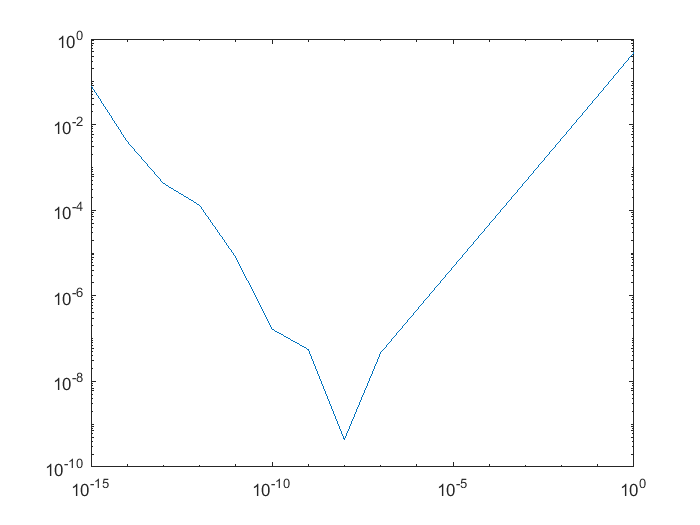
\includegraphics[scale=0.45]{1_1.png}
    \caption{向前差分精度随离散区间大小h的变化的情况}
\end{figure}
        \item(10分)推导出使用Richardson外推技术的向前差商的计算公式并用伪代码 给出算法。
    \item(5分)使用你的算法计算 $f(x)=\sin (x)$ 在 $x=1.2$ 处的导数并使用semilogy图 展示其精度随外推次数变化的情况。请自己选取h初始值,使得用外推方法
    能够算出的最精确的导数尽量精确。你的回答需要说明你使用外推方法算出
    的导数值是多少、误差又是多少、h的初始值是多少、外推了多少次。
    \end{enumerate}
    \item[第二题] 本题讨论使用复化梯形公式求周期函数的积分。
    \begin{enumerate}
        \item 
        (10分)证明当 $r$ 不是 $m$ 的整倍数的情况下,使用 $m$ 个子区间的复化梯形公式
        可以精确积分
        $$
        \int_{-\pi}^{\pi} \cos (r x) d x \quad \text { 和 } \quad \int_{-\pi}^{\pi} \sin (r x) d x
        $$
        注意:这一结论类似于课堂上我们定义的代数精度。同时说明如果 $r$ 为 $m$ 的
        整倍数时复化梯形公式对于上面两个积分会给出怎样的结果
        \item (10分)由于任意的以 $2 \pi$ 为周期的周期函数都可以表示为由正弦与余弦函数 的线性组合,所以上一问中所证明的定理实际上告诉我们求解一个周期函 数的积分的有效方法正是复化梯形公式。现使用复化梯形公式和不同数量 的子区间个数来求 $f(x)=e^{\cos (x)}$ 在 $[-\pi, \pi]$ 的积分,并用这个函数的真实积分 值作为参照使用semilogy图画出随着子区间数量 $m$ 变化所得到的积分精度 的变化。
        \par 题后语: 复化梯形公式之于周期函数的积分如同Gauss积分公式之于非周期
        函数的基于多项式的积分。因此复化梯形公式是最有效的求解周期函数积分 的方法。
    \end{enumerate} 
    \item[第三题] 
    \begin{enumerate}
        \item (10分)推导出如下格式的多步法公式:
        \begin{equation}\label{1}
            y_{n+1}=y_{n-1}+\alpha f_{n+1}+\beta f_{n}+\gamma f_{n-1}
        \end{equation}
        \item (10分)推导此格式的局部截断误差,并由此指明此格式的阶数。
        \item (10分)选取合适的步长值,用此格式在 $[0,2]$ 上解如下的初值问题:
        \begin{equation}\label{2}
            y^{\prime}=x e^{-4 x}-4 y, \quad y(0)=0
        \end{equation}

        使用你刚刚推导出的格式\ref{1},并利用二阶Runge-Kutta方法(即课本公式(7.15))起 步。画出解函数。
        \item (10分)推导出 \ref{2}的精确解。对比该精确解在 $x=2$ 这一点的值,用log-log图 展示所用方法的阶数,并给出解释。
    \end{enumerate}  
\end{enumerate}


\end{document}
